\section{Enaxliga problem}

\paragraph{Krafter på en stång}
Betrakta en stång med tvärsnittsarea $A$ som utsätts för en kraft $P$ i varje ända, med motsatt riktning i varje ända, som visad i figur \ref{fig:cylinder_forces}.
\begin{figure}[!ht]
	\centering
	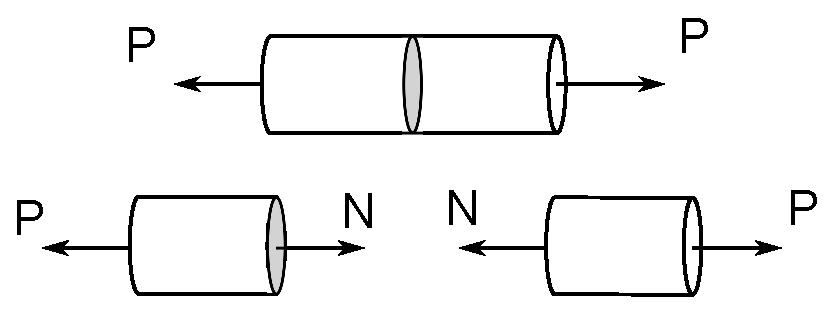
\includegraphics[width = 0.5\textwidth]{./Images/cylinder_forces.eps}
	\caption{Illustration av en stång som utsätts för en dragkraft och de orsakade inre krafterna.}
	\label{fig:cylinder_forces}
\end{figure}

Kraften $P$ i änderna propageras som inre krafter i stången. Om vi betraktar det indikerade tvärsnittet, manifesteras den inre kraften som en normalkraft på varje halva. Om vi definierar positiv riktning för normalkraften och dragkraften som i figuren, ger kraftjämvikten att $N = P$. Om dragkraften blir en tryckkraft, ändrar givetvis normalkraften riktning.

\paragraph{Spänning}
I hållfasthetslära är vi intresserade av påkänningen på materialet. Den beror av beloppet av normalkraften, men kan även spridas ut över tvärsnittet. Därför definierar vi spänningen
\begin{align*}
	\sigma = \frac{N}{A}.
\end{align*}
Jämvikten från innan ger
\begin{align*}
	\sigma = \frac{P}{A}.
\end{align*}

\paragraph{Deformation}
När en stång utsätts för spänning, kommer den att deformeras. Mer specifikt kommer den förlängas med en längd $\delta$. Eftersom förlängningen av varje del kommer från kraftjämvikten mellan normalkraften och dragkraften, kommer förlängningen för en given dragkraft bero av längden. Vi definierar därför töjningen
\begin{align*}
	\varepsilon	= \frac{\delta}{L_{0}}
\end{align*}
där $L_{0}$ är stångens ursprungliga längd.

\paragraph{Typer av samband i hållfasthetslära}
I hållfasthetsläran har vi tre typer av samband:
\begin{itemize}
	\item samband mellan krafter.
	\item samband mellan deformationer.
	\item konstitutiva samband (beskrivar materialbeteende).
\end{itemize}

\paragraph{Hookes lag}
Om man gör dragningsprov på olika material för små deformationer, blir plottet av $\sigma$ mot $\varepsilon$ approximativt linjär. Från detta får vi Hookes lag:
\begin{align*}
	\sigma = E\varepsilon.
\end{align*}
$E$ är elasticitetsmodulen, och beskrivar hur styvt materialet är. Från detta kan vi få
\begin{align*}
	P = \frac{EA}{L}\delta
\end{align*}
för en stång.

\paragraph{Normalspänning}
Vi utvidgar våran definition av spänning till spänningar som fördelas inhomogent över tvärsnittet vid att betrakta en inre kraft $\Delta F$ som verkar på ett arealement $\Delta A$, med riktningar som tidigare. Då definieras normalspänningen som
\begin{align*}
	\sigma = \lim\limits_{\Delta A\to 0}\frac{\Delta F}{\Delta A}.
\end{align*}

\paragraph{Normaltöjning}
Vi utvidgar även definitionen av töjning till töjningar som fördelas ojämnt över stavens längd. Om deformationen i en punkt är $u(x)$, ges töjningen av ett litet element med längd $\Delta x$ av
\begin{align*}
	\varepsilon = \lim\limits_{\Delta x\to 0}\frac{u(x + \Delta x) - u(x)}{\Delta x} = \dv{u}{x}.
\end{align*}

\paragraph{Tvärkontraktion}
När man gör ett dragningsprov på en stång, genomgår den deformation i längdriktning samtidigt som tjockleken minskar. Detta kallas tvärkontraktion. Töjningen $\varepsilon_{t}$ av tjockleken är relaterad till töjningen i längdriktning genom
\begin{align*}
	\varepsilon_{t} = -v\varepsilon,
\end{align*}
där $v$ är Poissons konstant.